% IEEEAerospace2012.cls requires the following packages: times, rawfonts, oldfont, geometry
\documentclass[twocolumn,letterpaper]{article}  % only supports two-column, letterpaper format

\usepackage{booktabs}
\usepackage[]{graphicx,latexsym,amssymb,amsfonts,amsmath,amstext,times}
% NOTE: The .cls file is now compatible with amsmath!!!

\usepackage{floatrow}
\usepackage{hyperref}

\newcommand{\ignore}[1]{}  % {} empty inside = %% comment
\usepackage{enumitem}
\setlist[itemize]{leftmargin=*}
\setlist[enumerate]{leftmargin=*}

% Default fixed font does not support bold face
\DeclareFixedFont{\ttb}{T1}{txtt}{bx}{n}{12} % for bold
\DeclareFixedFont{\ttm}{T1}{txtt}{m}{n}{12}  % for normal

% Custom colors
\usepackage{color}
\usepackage{listings}
\usepackage{framed}
\usepackage{caption}
\usepackage{bm}
\captionsetup[lstlisting]{font={small,tt}}

\definecolor{mygreen}{rgb}{0,0.6,0}
\definecolor{mygray}{rgb}{0.5,0.5,0.5}
\definecolor{mymauve}{rgb}{0.58,0,0.82}

\lstset{ %
  backgroundcolor=\color{white},   % choose the background color; you must add \usepackage{color} or \usepackage{xcolor}
  basicstyle=\ttfamily\footnotesize, % the size of the fonts that are used for the code
  breakatwhitespace=false,         % sets if automatic breaks should only happen at whitespace
  breaklines=true,                 % sets automatic line breaking
  captionpos=b,                    % sets the caption-position to bottom
  commentstyle=\color{mygreen},    % comment style
  deletekeywords={...},            % if you want to delete keywords from the given language
  escapeinside={\%*}{*)},          % if you want to add LaTeX within your code
  extendedchars=true,              % lets you use non-ASCII characters; for 8-bits encodings only, does not work with UTF-8
  frame=single,                    % adds a frame around the code
  keepspaces=true,                 % keeps spaces in text, useful for keeping indentation of code (possibly needs columns=flexible)
  columns=flexible,
  keywordstyle=\color{blue},       % keyword style
  language=Python,                 % the language of the code
  morekeywords={*,...},            % if you want to add more keywords to the set
  numbers=left,                    % where to put the line-numbers; possible values are (none, left, right)
  numbersep=5pt,                   % how far the line-numbers are from the code
  numberstyle=\tiny\color{mygray}, % the style that is used for the line-numbers
  rulecolor=\color{black},         % if not set, the frame-color may be changed on line-breaks within not-black text (e.g. comments (green here))
  showspaces=false,                % show spaces everywhere adding particular underscores; it overrides 'showstringspaces'
  showstringspaces=false,          % underline spaces within strings only
  showtabs=false,                  % show tabs within strings adding particular underscores
  stepnumber=1,                    % the step between two line-numbers. If it's 1, each line will be numbered
  stringstyle=\color{mymauve},     % string literal style
  tabsize=4,                       % sets default tabsize to 2 spaces
}
\usepackage{epigraph}
\renewcommand{\textflush}{flushepinormal}

\begin{document}

\title{Extra Credit - RPG Dice Simulator}
\author{%
John Karasinski\\
karasinski@gmail.com
}
\date{}

\maketitle

\thispagestyle{plain}
\pagestyle{plain}

%%%%%%%%%%%%%%%%%%%%%%%%%%%%%%%%%%%%%%
\section{Introduction}
%%%%%%%%%%%%%%%%%%%%%%%%%%%%%%%%%%%%%%

\epigraph{\small\itshape God's dice always have a lucky roll.}{Sophocles (497/6 --- 406/5 BC)}%
\vspace{-2em}
\epigraph{\small\itshape God does not play dice.}{Albert Einstein (1879 --- 1955)}%
\vspace{-2em}
\epigraph{\small\itshape God not only plays dice, but also sometimes throws them where they cannot be seen.}{Stephen Hawking (1942 --- \hspace{1.5em})}%

While God's use of dice may be disputed, humans have been using dice in games of chance for many thousands of years~\cite{history}. Dice insert a certain amount of randomness into games, and can lead to wonderfully unpredictable situations. Perhaps more importantly, and in spite of the randomness associated with them, dice are also excellent for bringing everyone to the same level. A king and a peasant have the same odds of rolling a six, and the die does not care who is more wealthy, talented, or desperate. Despite their use for thousands of years, humans are very bad at predicting the outcomes of dice throws. Luckily, while the result of any individual roll of the die may be random and unknown, a basic application of statistics can lead us to make more informed decisions about the likelihood of events.

The only assumption going forward is that we are considering perfect dice. These perfect dice have the property of having an equal probability of landing on any particular face. According to standard die notation, die rolls are given in the form AdX. A and X are variables, separated by the letter ``d'', which stands for die or dice~\cite{dice_notation}. A six-sided die (1d6), for example, would then have a $1/6$ probability of resulting in a 1, 2, 3, 4, 5 or 6. Cheap dice purchased for gaming will not have this property, and will instead slightly favor different outcomes. For the purposes of the simulations here, you can assume that we have purchased \textit{very, very expensive} dice which behave perfectly.

%%%%%%%%%%%%%%%%%%%%%%%%%%%%%%%%%%%%%%
\section{Instructions}
%%%%%%%%%%%%%%%%%%%%%%%%%%%%%%%%%%%%%%
The project should consist of a brief write-up introducing relevant theory behind each simulation problem, your simulation method, your results, and a summary of your conclusions. I'm looking for short papers ranging 5-8 pages in length. These papers should focus on the simulation methodology and results, with these sections making up the bulk of the paper.\\

Create a function that will allow me to specify the number of dice I want to use per roll, the number of faces on each die (assume all dice used in a roll have the same number of faces), whether I will sum the scores of each die or will have a minimum value needed to count as a success per die, and whether I will include botches or not as an outcome for rolls.\\

Example requirements:%
\begin{enumerate}
\itemsep-.25em
\item Roll 1d20 and I just want to know the score.
\item Roll 2d6 and I want to know my summed scores.
\item Roll 4d10 where I need to roll 5s or greater such that each roll of 5 or greater counts as a success.
\item The same scenario as above, but now each 1 rolled detracts from the number of successes.
\end{enumerate}

%%%%%%%%%%%%%%%%%%%%%%%%%%%%%%%%%%%%%%
\section{Simulation Method}
%%%%%%%%%%%%%%%%%%%%%%%%%%%%%%%%%%%%%%

This simulation will make use of Python 3.5.0. The core idea behind the simulation is to generate pseudo-random numbers to simulate the throwing of many dice. From there, the rules given in the problem prompt can be applied to deduce the result of the throw.

The basic functionality behind the simulation is the \texttt{dice()} function. This function accepts three arguments, \texttt{A}, \texttt{X}, and an optional \texttt{n}, where \texttt{A} and \texttt{X} take on the same meaning as in standard dice notation, and n is the number of times to simulate the throw. Calling \texttt{dice(3, 6, n=2)}, for example, would return \texttt{array([[2, 2, 6], [5, 3, 4]])}. This array has 2 rows of 3 simulated 6-sided dice.

The \texttt{dice()} function is essentially a helper function, which calls Numpy's random integer function. Numpy uses the Mersenne twister sequence to generate random numbers. As these are psuedo-random numbers and not true random numbers, knowing the seed of the algorithm allows you to reproduce the results, and predict future events with 100\% accuracy.

%%%%%%%%%%%%%%%%%%%%%%%%%%%%%%%%%%%%%%
\section{Results}
%%%%%%%%%%%%%%%%%%%%%%%%%%%%%%%%%%%%%%

a. Roll 1d6 1,000 times, frequency of each outcome?
\begin{figure}%[h!]
\centering
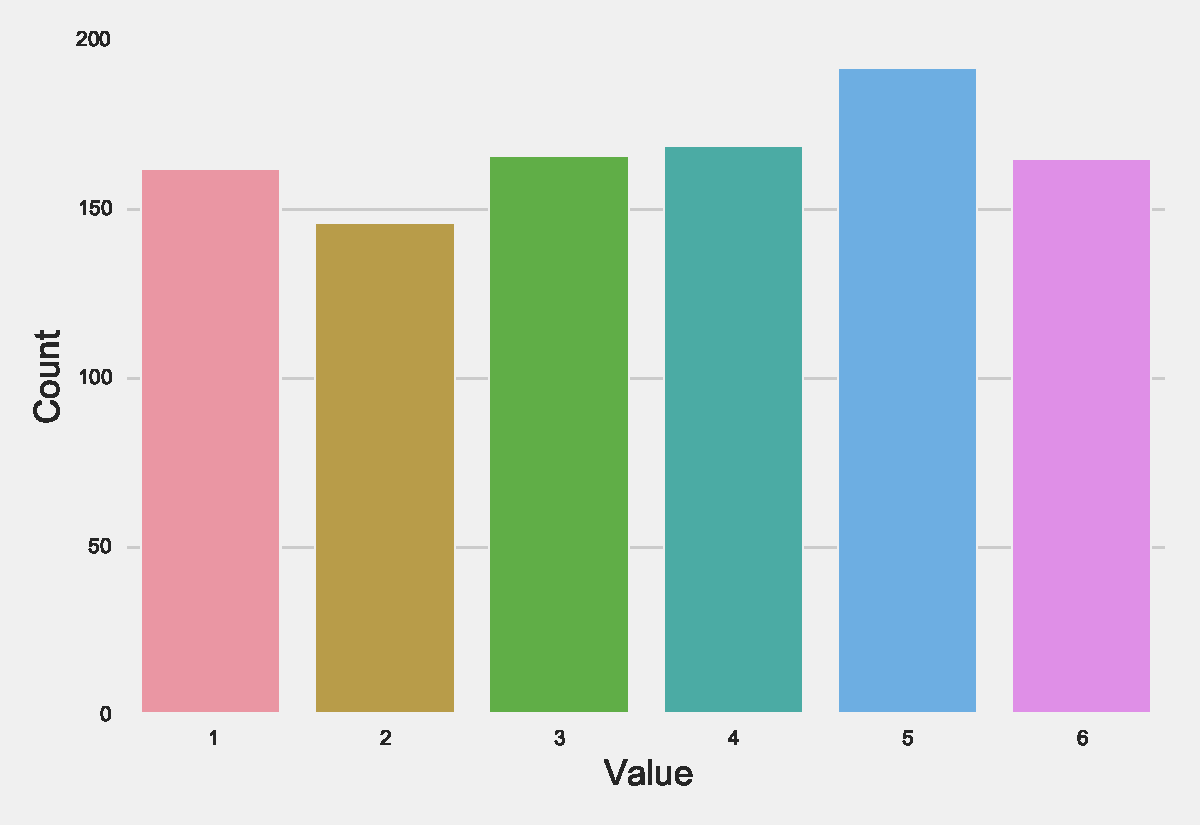
\includegraphics[width=3.25in]{1d6.pdf}
\caption{Results from 1,000 1d6 rolls.}
% \label{fig:on}
\end{figure}

\begin{table}%[h!]
\begin{center}
\begin{tabular}{*{3}{r}}
\toprule
Value & Count & Frequency \\
\midrule
 1   & 173      & 17.3 \\
 2   & 182      & 18.2 \\
 3   & 163      & 16.3 \\
 4   & 147      & 14.7 \\
 5   & 156      & 15.6 \\
 6   & 179      & 17.9 \\
\bottomrule
\end{tabular}
\end{center}
\caption{Results of 1,000 1d6 rolls}
\end{table}

b. Roll 2d6 1,000 times, frequency of each outcome? Use the summed scores of each die as your outcome.
\begin{figure}%[h!]
\centering
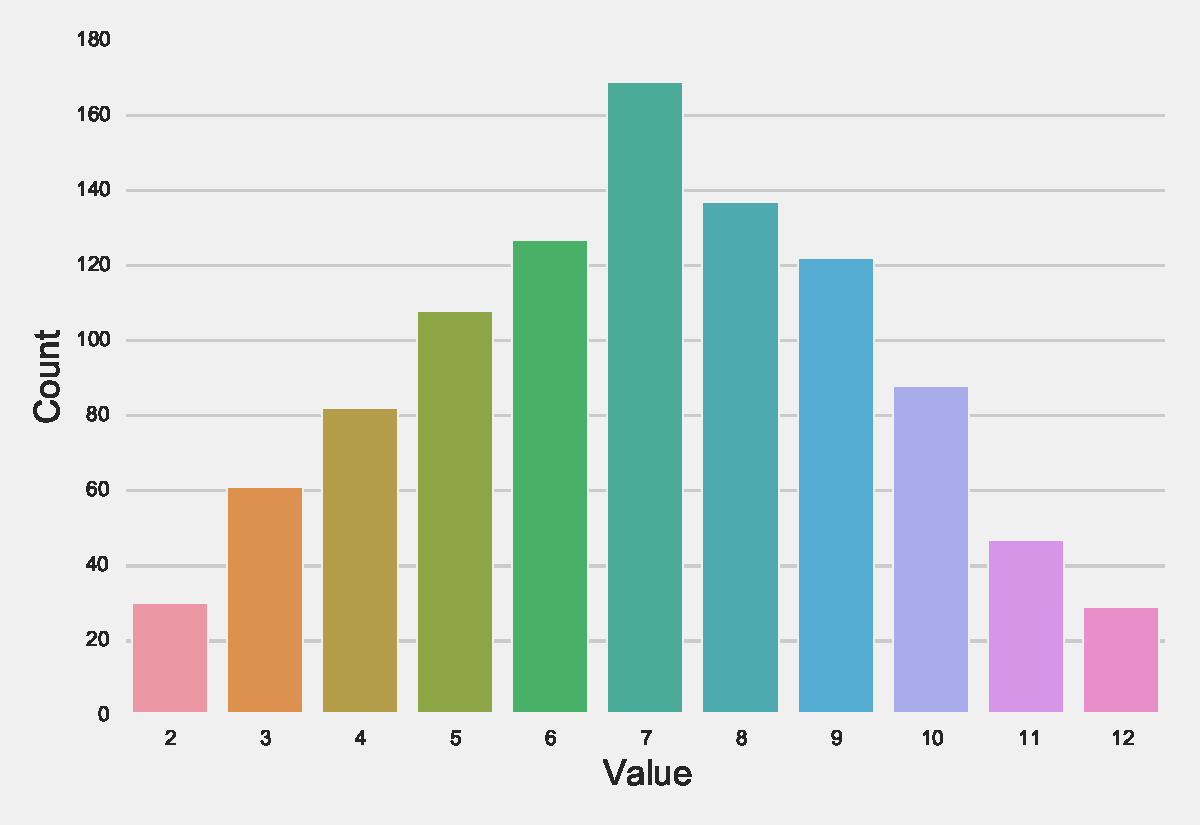
\includegraphics[width=3.25in]{2d6.pdf}
\caption{Results of summed values from 1,000 2d6 rolls.}
% \label{fig:on}
\end{figure}

\begin{table}%[h!]
\begin{center}
\begin{tabular}{*{3}{r}}
\toprule
Value & Count & Frequency \\
\midrule
 2   &  30      &  3.0 \\
 3   &  61      &  6.1 \\
 4   &  82      &  8.2 \\
 5   & 108      & 10.8 \\
 6   & 127      & 12.7 \\
 7   & 169      & 16.9 \\
 8   & 137      & 13.7 \\
 9   & 122      & 12.2 \\
10   &  88      &  8.8 \\
11   &  47      &  4.7 \\
12   &  29      &  2.9 \\
\bottomrule
\end{tabular}
\end{center}
\caption{Results of summed values from 1,000 2d6 rolls.}
\end{table}

c. Roll 6d10 1,000 times, frequency of each outcome? Treat a score of 6 or better as a success and scores less than 6 as nothing, the outcome is total number of successes (include the frequency of no successes).
\begin{figure}%[h!]
\centering
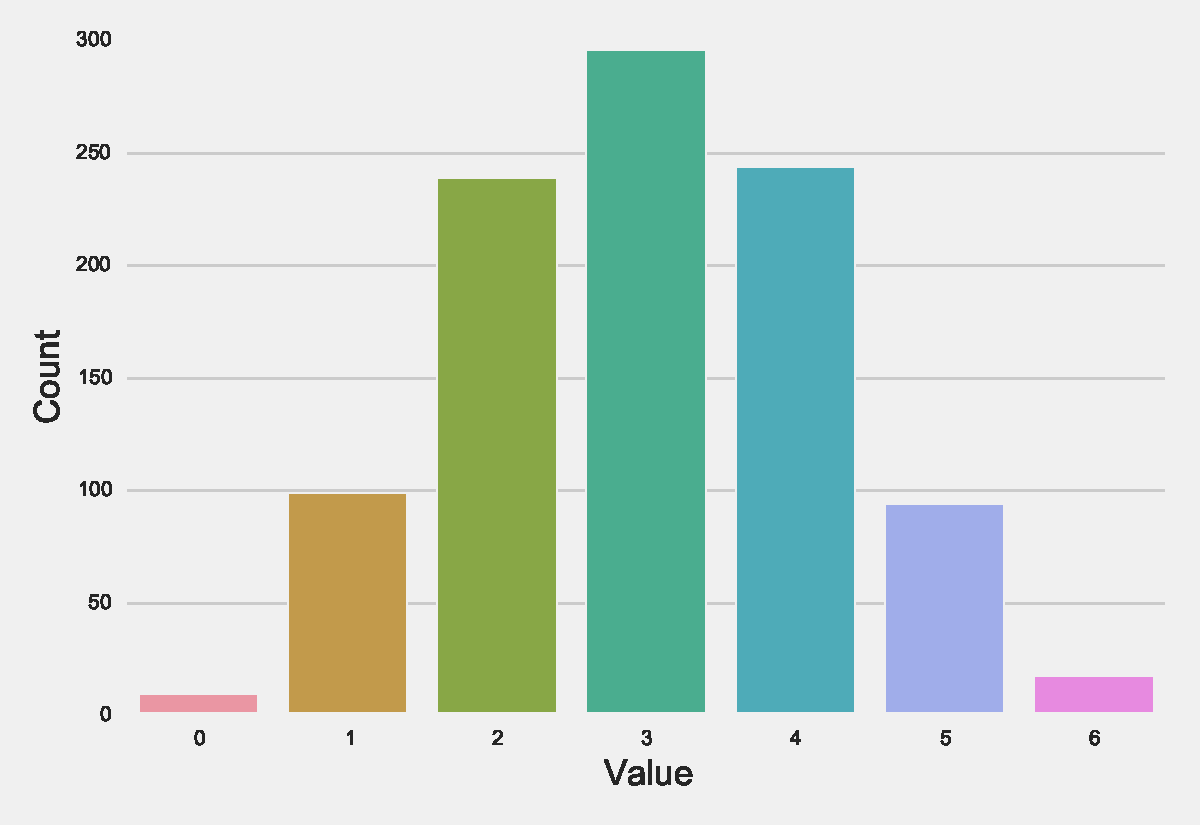
\includegraphics[width=3.25in]{6d10>6.pdf}
\caption{Results of succeses from 1,000 6d10 rolls, where scores of 6 or greater are considered successes.}
% \label{fig:on}
\end{figure}

\begin{table}%[h!]
\begin{center}
\begin{tabular}{*{3}{r}}
\toprule
Value & Count & Frequency \\
\midrule
0   &  10      &  1.0 \\
1   &  99      &  9.9 \\
2   & 239      & 23.9 \\
3   & 296      & 29.6 \\
4   & 244      & 24.4 \\
5   &  94      &  9.4 \\
6   &  18      &  1.8 \\
\bottomrule
\end{tabular}
\end{center}
\caption{Results of succeses from 1,000 6d10 rolls, where scores of 6 or greater are considered successes.}
\end{table}

d. Same as (c) above except now scores of 1 count as a botch. Each botch is subtracted from each success. If there are more botches than success (i.e., -1 successes) then the overall outcome is a botch. Now depict the frequency of botching, and total number of successes (as before, include the frequency of no successes).
\begin{figure}%[h!]
\centering
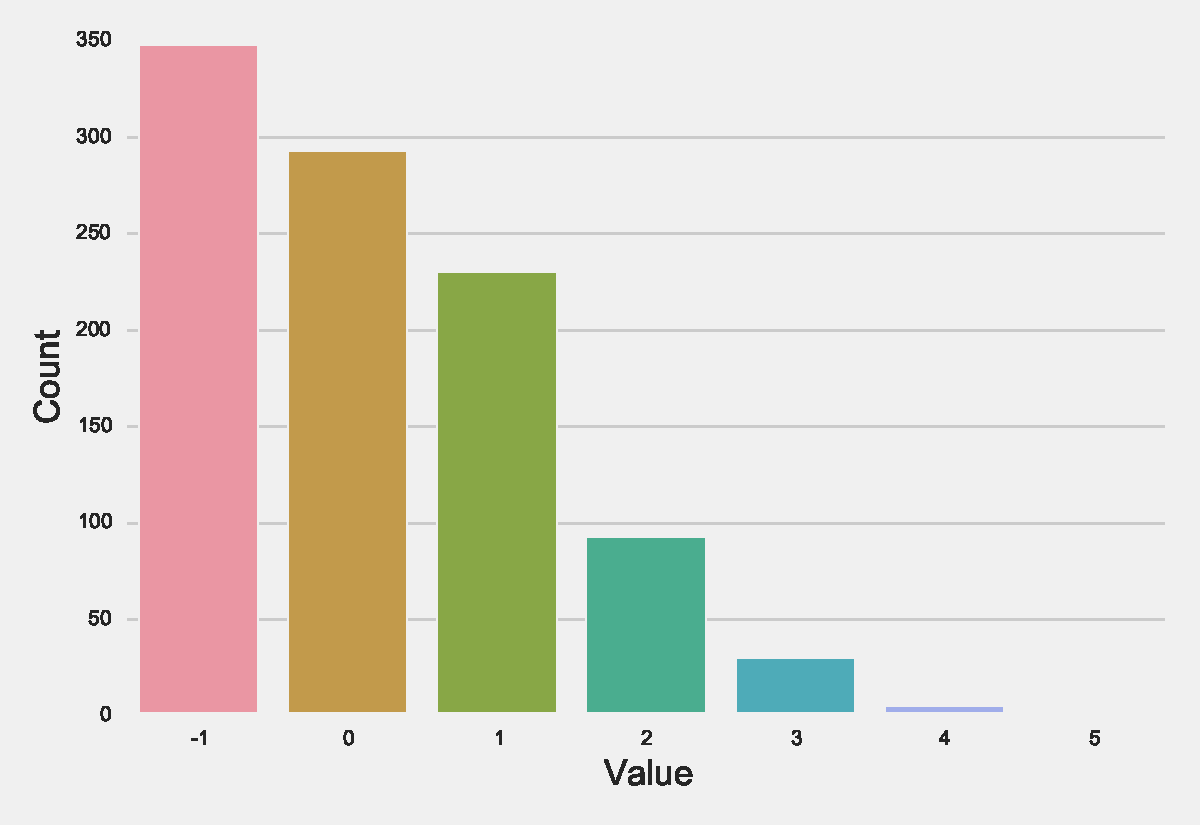
\includegraphics[width=3.25in]{6d10>6-botching.pdf}
\caption{Results of succeses from 1,000 6d10 rolls, where scores of 6 or greater are considered successes, and scores of 1 are considered botches.}
% \label{fig:on}
\end{figure}

\begin{table}%[h!]
\begin{center}
\begin{tabular}{*{3}{r}}
\toprule
Value & Count & Frequency \\
\midrule
 -1   & 348      & 34.8 \\
  0   & 293      & 29.3 \\
  1   & 230      & 23.0 \\
  2   &  93      &  9.3 \\
  3   &  30      &  3.0 \\
  4   &   5      &  0.5 \\
  5   &   1      &  0.1 \\
\bottomrule
\end{tabular}
\end{center}
\caption{Results of succeses from 1,000 6d10 rolls, where scores of 6 or greater are considered successes, and scores of 1 are considered botches.}
\end{table}

%%%%%%%%%%%%%%%%%%%%%%%%%%%%%%%%%%%%%%
\section{Summary}
%%%%%%%%%%%%%%%%%%%%%%%%%%%%%%%%%%%%%%


\bibliographystyle{IEEEtran}
%\bibliography{IEEEabr,MyBle}
\begin{thebibliography}{1}

\bibitem{history}
Carlisle, Rodney P., ed. Encyclopedia of play in today's society. Vol. 1. Sage, 2009.

\bibitem{dice_notation}
``Standard Dice Notation''. dice-play. 2006-04-06. Archived from the original on 2007-04-26. https://web.archive.org/web/20070426013749/http://homepage.ntlworld.com/dice-play/Notation.htm

\end{thebibliography}

\clearpage
\onecolumn
%%%%%%%%%%%%%%%%%%%%%%%%%%%%%%%%%%%%%%%%%%%%%%%%%%%%%%%%%%%%%%%%%%%%%%%%%%%%%%%%%%%%%%%%%%%%%%%%%
\appendix{}               % note there is no {} to put a title. Each appendix has its own title
%%%%%%%%%%%%%%%%%%%%%%%%%%%%%%%%%%%%%%%%%%%%%%%%%%%%%%%%%%%%%%%%%%%%%%%%%%%%%%%%%%%%%%%%%%%%%%%%%
% For a single appendix, use the \appendix{} keyword and do not use the \section command.

\section{Source Code}        % first appendix
\lstinputlisting{"../Option 1 Computation/dice.py"}
% %%%%%%%%%%%%%%%%%%%%%%%%%%
% This is the first appendix.

% \subsection{Comments}
% If you have only one appendix, use the ``appendix'' keyword.

% \subsection{More Comments}
% Use section and subsection keywords as usual.

\end{document}

